\documentclass{beamer}
\usepackage{fontawesome5}
\usepackage{physics}
\usepackage{amsmath}
\usepackage{tikz}
\usepackage{mathdots}
\usepackage{mathtools}
\usepackage{yhmath}
\usepackage[version=4]{mhchem}
\usepackage{cancel}
\usepackage{color}
\usepackage{siunitx}
\usepackage{array}
\usepackage{multirow}
\usepackage{graphicx}
\usepackage{amssymb}
\usepackage{pifont}
\newcommand{\cmark}{\ding{51}}%
\newcommand{\xmark}{\ding{55}}%
\usepackage{textcomp, gensymb}
\usepackage{tabularx}
\usepackage{extarrows}
\usepackage{booktabs}
\usetikzlibrary{fadings}
\usetikzlibrary{patterns}
\usetikzlibrary{shadows.blur}
\usetikzlibrary{shapes}
\usepackage[style=authoryear,backend=bibtex]{biblatex}
\addbibresource{arpes.bib}
\addbibresource{green.bib}
\addbibresource{material.bib}
\addbibresource{monolayer-WTe2.bib}
\addbibresource{topological}
\addbibresource{exciton-insulator}
\usepackage{listings}
\usepackage{hyperref}

\newcommand{\pair}[1]{\langle #1 \rangle}
\DeclareMathOperator{\ee}{e}
\DeclareMathOperator{\ii}{i}
\DeclareMathOperator{\sgn}{sgn}
\newcommand{\shortcode}[1]{\texttt{#1}}

% Displaying texts in bookmarkers

\pdfstringdefDisableCommands{%
  \def\\{}%
  \def\ce#1{<#1>}%
}

\pdfstringdefDisableCommands{%
  \def\texttt#1{<#1>}%
  \def\mathbb#1{#1}%
}
\pdfstringdefDisableCommands{\def\eqref#1{(\ref{#1})}}

\makeatletter
\pdfstringdefDisableCommands{\let\HyPsd@CatcodeWarning\@gobble}
\makeatother

%Information to be included in the title page:
\title{Band theory}
\author{Jinyuan Wu}

\usetheme{Madrid}

\begin{document}

\frame{\titlepage}

\begin{frame}
\frametitle{Matter = Nuclei + electrons}

\begin{center}
    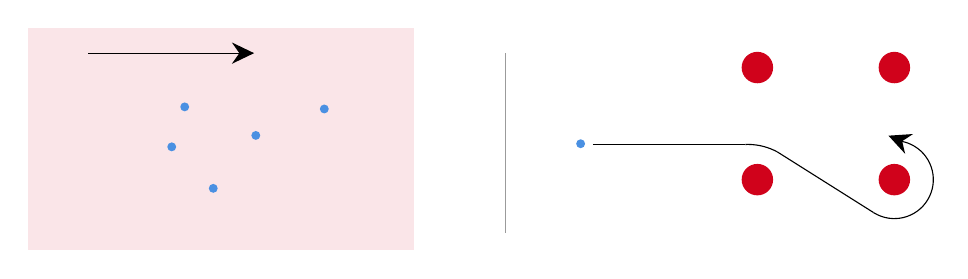
\begin{tikzpicture}[x=0.75pt,y=0.75pt,yscale=-1,xscale=1]
        %uncomment if require: \path (0,300); %set diagram left start at 0, and has height of 300
        
        %Shape: Rectangle [id:dp5203758107088254] 
        \draw  [draw opacity=0][fill={rgb, 255:red, 208; green, 2; blue, 27 }  ,fill opacity=0.1 ] (53,83) -- (238.83,83) -- (238.83,189.85) -- (53,189.85) -- cycle ;
        %Shape: Circle [id:dp2638771131786344] 
        \draw  [draw opacity=0][fill={rgb, 255:red, 74; green, 144; blue, 226 }  ,fill opacity=1 ] (120,140.15) .. controls (120,138.96) and (120.96,138) .. (122.15,138) .. controls (123.33,138) and (124.29,138.96) .. (124.29,140.15) .. controls (124.29,141.33) and (123.33,142.29) .. (122.15,142.29) .. controls (120.96,142.29) and (120,141.33) .. (120,140.15) -- cycle ;
        %Straight Lines [id:da8498772044832128] 
        \draw    (82,95) -- (158.83,95) ;
        \draw [shift={(161.83,95)}, rotate = 180] [fill={rgb, 255:red, 0; green, 0; blue, 0 }  ][line width=0.08]  [draw opacity=0] (10.72,-5.15) -- (0,0) -- (10.72,5.15) -- (7.12,0) -- cycle    ;
        %Shape: Circle [id:dp5206870381778301] 
        \draw  [draw opacity=0][fill={rgb, 255:red, 208; green, 2; blue, 27 }  ,fill opacity=1 ] (462.73,155.94) .. controls (462.73,151.76) and (466.12,148.37) .. (470.3,148.37) .. controls (474.48,148.37) and (477.88,151.76) .. (477.88,155.94) .. controls (477.88,160.13) and (474.48,163.52) .. (470.3,163.52) .. controls (466.12,163.52) and (462.73,160.13) .. (462.73,155.94) -- cycle ;
        %Shape: Circle [id:dp6691480595148553] 
        \draw  [draw opacity=0][fill={rgb, 255:red, 74; green, 144; blue, 226 }  ,fill opacity=1 ] (140,160.15) .. controls (140,158.96) and (140.96,158) .. (142.15,158) .. controls (143.33,158) and (144.29,158.96) .. (144.29,160.15) .. controls (144.29,161.33) and (143.33,162.29) .. (142.15,162.29) .. controls (140.96,162.29) and (140,161.33) .. (140,160.15) -- cycle ;
        %Shape: Circle [id:dp2337212483051676] 
        \draw  [draw opacity=0][fill={rgb, 255:red, 74; green, 144; blue, 226 }  ,fill opacity=1 ] (160.5,134.65) .. controls (160.5,133.46) and (161.46,132.5) .. (162.65,132.5) .. controls (163.83,132.5) and (164.79,133.46) .. (164.79,134.65) .. controls (164.79,135.83) and (163.83,136.79) .. (162.65,136.79) .. controls (161.46,136.79) and (160.5,135.83) .. (160.5,134.65) -- cycle ;
        %Shape: Circle [id:dp47231302420761323] 
        \draw  [draw opacity=0][fill={rgb, 255:red, 74; green, 144; blue, 226 }  ,fill opacity=1 ] (126.25,120.9) .. controls (126.25,119.71) and (127.21,118.75) .. (128.4,118.75) .. controls (129.58,118.75) and (130.54,119.71) .. (130.54,120.9) .. controls (130.54,122.08) and (129.58,123.04) .. (128.4,123.04) .. controls (127.21,123.04) and (126.25,122.08) .. (126.25,120.9) -- cycle ;
        %Shape: Circle [id:dp38473573369680714] 
        \draw  [draw opacity=0][fill={rgb, 255:red, 74; green, 144; blue, 226 }  ,fill opacity=1 ] (193.5,121.9) .. controls (193.5,120.71) and (194.46,119.75) .. (195.65,119.75) .. controls (196.83,119.75) and (197.79,120.71) .. (197.79,121.9) .. controls (197.79,123.08) and (196.83,124.04) .. (195.65,124.04) .. controls (194.46,124.04) and (193.5,123.08) .. (193.5,121.9) -- cycle ;
        %Shape: Circle [id:dp05721063166364493] 
        \draw  [draw opacity=0][fill={rgb, 255:red, 74; green, 144; blue, 226 }  ,fill opacity=1 ] (317,138.65) .. controls (317,137.46) and (317.96,136.5) .. (319.15,136.5) .. controls (320.33,136.5) and (321.29,137.46) .. (321.29,138.65) .. controls (321.29,139.83) and (320.33,140.79) .. (319.15,140.79) .. controls (317.96,140.79) and (317,139.83) .. (317,138.65) -- cycle ;
        %Straight Lines [id:da6807525071286458] 
        \draw    (325,139) -- (398.48,139) ;
        %Shape: Arc [id:dp4390049795383295] 
        \draw  [draw opacity=0] (398.48,139) .. controls (398.99,138.98) and (399.5,138.97) .. (400.01,138.98) .. controls (405.08,139.04) and (409.83,140.36) .. (413.99,142.63) -- (399.64,168.98) -- cycle ; \draw   (398.48,139) .. controls (398.99,138.98) and (399.5,138.97) .. (400.01,138.98) .. controls (405.08,139.04) and (409.83,140.36) .. (413.99,142.63) ;  
        %Straight Lines [id:da48988805092708443] 
        \draw    (413.99,142.63) -- (460.21,171.77) ;
        %Shape: Arc [id:dp5214021465034457] 
        \draw  [draw opacity=0] (473.92,137.52) .. controls (476.01,137.93) and (478.07,138.71) .. (480,139.87) .. controls (488.88,145.23) and (491.73,156.77) .. (486.37,165.64) .. controls (481.02,174.52) and (469.48,177.37) .. (460.6,172.02) .. controls (460.47,171.94) and (460.34,171.85) .. (460.21,171.77) -- (470.3,155.94) -- cycle ; \draw   (473.92,137.52) .. controls (476.01,137.93) and (478.07,138.71) .. (480,139.87) .. controls (488.88,145.23) and (491.73,156.77) .. (486.37,165.64) .. controls (481.02,174.52) and (469.48,177.37) .. (460.6,172.02) .. controls (460.47,171.94) and (460.34,171.85) .. (460.21,171.77) ;  
        %Straight Lines [id:da4943017179285871] 
        \draw    (471.21,136.27) -- (470.24,135.89) ;
        \draw [shift={(467.46,134.77)}, rotate = 21.8] [fill={rgb, 255:red, 0; green, 0; blue, 0 }  ][line width=0.08]  [draw opacity=0] (10.72,-5.15) -- (0,0) -- (10.72,5.15) -- (7.12,0) -- cycle    ;
        %Straight Lines [id:da13197145098593] 
        \draw [color={rgb, 255:red, 155; green, 155; blue, 155 }  ,draw opacity=1 ]   (283,95) -- (283,181.85) ;
        %Shape: Circle [id:dp8940324852277308] 
        \draw  [draw opacity=0][fill={rgb, 255:red, 208; green, 2; blue, 27 }  ,fill opacity=1 ] (396.73,155.94) .. controls (396.73,151.76) and (400.12,148.37) .. (404.3,148.37) .. controls (408.48,148.37) and (411.88,151.76) .. (411.88,155.94) .. controls (411.88,160.13) and (408.48,163.52) .. (404.3,163.52) .. controls (400.12,163.52) and (396.73,160.13) .. (396.73,155.94) -- cycle ;
        %Shape: Circle [id:dp032053078558565096] 
        \draw  [draw opacity=0][fill={rgb, 255:red, 208; green, 2; blue, 27 }  ,fill opacity=1 ] (462.73,101.94) .. controls (462.73,97.76) and (466.12,94.37) .. (470.3,94.37) .. controls (474.48,94.37) and (477.88,97.76) .. (477.88,101.94) .. controls (477.88,106.13) and (474.48,109.52) .. (470.3,109.52) .. controls (466.12,109.52) and (462.73,106.13) .. (462.73,101.94) -- cycle ;
        %Shape: Circle [id:dp6260109360185968] 
        \draw  [draw opacity=0][fill={rgb, 255:red, 208; green, 2; blue, 27 }  ,fill opacity=1 ] (396.73,101.94) .. controls (396.73,97.76) and (400.12,94.37) .. (404.3,94.37) .. controls (408.48,94.37) and (411.88,97.76) .. (411.88,101.94) .. controls (411.88,106.13) and (408.48,109.52) .. (404.3,109.52) .. controls (400.12,109.52) and (396.73,106.13) .. (396.73,101.94) -- cycle ;
        
        
        
        
        \end{tikzpicture}

\end{center}    

Paradox!

\end{frame}

\begin{frame}
\frametitle{Electrons as waves}



\end{frame}

\begin{frame}
\frametitle{The influence of crystal: ``band structure''}

    

\end{frame}

\end{document}